\documentclass{article}
\usepackage[english]{babel}
%\usepackage[utf8]{inputenc}
\usepackage{amsmath}
\usepackage{amsfonts}
\usepackage{amssymb}
\usepackage{graphicx}
\usepackage{float}
\usepackage{hyperref}
\usepackage{geometry}
\usepackage{titling}
\usepackage{csquotes}
\usepackage[]{biblatex}
\usepackage{titlesec}
\usepackage{listings}
\usepackage{xcolor}
\usepackage{multicol}
%\usepackage{fetamont}
%\usepackage{scrextend}
%\usepackage{fontspec}

%\setmonofont[Scale=0.9]{Fira Code Medium}
%\urlstyle{sf}

\addbibresource{citations.bib}

\geometry{a4paper, portrait, margin=5em, bmargin=10em, tmargin=10em,columnsep=20pt}

\titleclass{\subsubsubsection}{straight}[\subsection]

\newcounter{subsubsubsection}[subsubsection]
\renewcommand\thesubsubsubsection{\thesubsubsection.\arabic{subsubsubsection}}
\renewcommand\theparagraph{\thesubsubsubsection.\arabic{paragraph}} % optional; useful if paragraphs are to be numbered

\titleformat{\subsubsubsection}
  {\normalfont\normalsize\bfseries}{\thesubsubsubsection}{1em}{}
\titlespacing*{\subsubsubsection}
{0pt}{2ex plus 1ex minus .2ex}{1.5ex plus .2ex}

\makeatletter
\def\toclevel@subsubsubsection{4}
\def\l@subsubsubsection{\@dottedtocline{4}{7em}{4em}}
\makeatother

\setcounter{secnumdepth}{4}
\setcounter{tocdepth}{4}

\setlength{\droptitle}{-5em} %-5em
\newcommand{\spc}{\:}
\newcommand{\constraint}[4]{(#1,\spc #2,\spc #3,\spc #4)}
\newcommand{\plchold}[1]{\texttt{\textit{<#1>}}}
\newcommand{\mathplchold}[1]{\text{\texttt{\textit{<#1>}}}}
\newcommand{\linenum}[1]{\texttt{#1}}

\definecolor{background}{HTML}{F4F4F4}
\definecolor{keyword}{HTML}{B23E72}
\definecolor{string}{HTML}{E56916}
\definecolor{variables}{HTML}{6B70D6}
\definecolor{comments}{HTML}{4F993D}
\definecolor{gutter}{HTML}{B2B2B2}

\lstset{
    % Background color
	backgroundcolor=\color{background},
	% Comments style
	commentstyle=\color{comments},
	% Gutter color
	fillcolor=\color{gutter},
	rulecolor=\color{gutter},
	% Keywords style
	keywordstyle=\color{keyword},
	% String style
	stringstyle=\color{string},
	% Code style
	basicstyle=\ttfamily\footnotesize,
	numberstyle=\ttfamily,
	breakatwhitespace=true,
	breaklines=true,                 % sets automatic line breaking
	keepspaces=true, 
	stepnumber=1,
	tabsize=4,
	% Frame
	frame=l,
	%framerule=4mm,
	xleftmargin=0.65cm,
	framesep=4.5mm,
	framexleftmargin=1.5mm,
	numbersep=6pt,
	numbers=left,
	% Language-specific style
	language={Java},
	classoffset=0,
	keywordstyle=\color{keyword},       % keyword style
	morekeywords={def},
	keywordstyle=\color{keyword},
	classoffset=1,
	morekeywords={a, b, c, d, e, f, g},
	keywordstyle=\color{variables},
}

\title{\Huge
%\Large Software Correctness, Security and Reliability Project Report\\[1em]
%\large Stripes Domain
\textbf{Stripes Domain}\\[0.5em]
\large  Software Correctness, Security and Reliability Project Report
}
\author{\large Alessio De Biasi\\ 
        \normalsize Ca’ Foscari University of Venice, Italy\\
        \normalsize 870288@stud.unive.it
        \and
        \large Jonathan Gobbo\\
        \normalsize Ca’ Foscari University of Venice, Italy\\
        \normalsize 870506@stud.unive.it
}
\date{}

\begin{document}
\twocolumn
\maketitle



%\tableofcontents


\section{Introduction}

The purpose of this project is to implement in LiSA \cite{lisa}, a library for static analysis developed by the group \citeauthor{lisa},  the Stripes abstract domain.
This domain is originally proposed in the paper \citetitle{ferrara} \cite{ferrara} by \citeauthor{ferrara}.

The authors propose this domain in order to analyze unsafe C\# code in which unsafe operations, such as manipulating pointers or performing arbitrary casts, are allowed.

In this case, the usual run-time bound checking is not performed, meaning that the programmer can involuntary cause a wide range of errors, such as buffer and array overflows.

The Stripes abstract domain is therefore used to statically verify memory accesses, in such a way that upper bounds of allocated memory are not exceeded.


\section{Formal definition}
%       Tracciare vincoli z-k1*....
%       Perchè ? (Idea dell'articolo sizeof(T))
%       Applicazioni, a che serve
%       Limiti (solo upper bound)
% FORSE ----> LUB, Less or equal, Widening

The Stripes abstract domain tracks constraints in the form:
\begin{equation}
\label{constr_formula}
    x - k_1\cdot(y\ [+z]) > k_2
\end{equation}
\noindent
where $x$, $y$ and $z$ (which is optional) are variables, while $k_1$ and $k_2$ are integer constants.
% TODO Riformulare
Since in a program the only statements that can be expressed in this form are assignments and boolean conditions, only such statements are analyzed.


\subsection{Domain representation}
The elements in the Stripes abstract domain are represented by a map from variables to constraints.
In particular, each constraint in the normalized form (see equation \ref{constr_formula}) is represented by a quadruple $(y,\spc z,\spc k_1,\spc k_2)$.

If $z$ is absent, the constraint is represented, instead, by the quadruple $(y,\spc \perp,\spc k_1,\spc k_2)$. 

Formally, let $\mathcal{V}$ be the set of all the variables in the analyzed program. A Stripes abstract domain element is the map:
$$
\Big[\mathcal{V} \rightarrow \mathcal{P}\big((\mathcal{V} \times (\mathcal{V}\ \cup \perp) \times \mathbb{N} \times \mathbb{N})\big)\Big]
$$

The top domain element $\top$ expresses the fact that the abstract state tracks no variables.

The bottom domain element $\perp$, instead, expresses the fact that the abstract state contains a contradiction (i.e., the statement, to which the $\perp$ domain element is associated to, is not reachable at run-time, whatever execution path the program takes).

\subsection{Assignments}
% Tracciamo trinomio (3 monomi): due var e una const
% da = a >= e dopo > 
% Nuovi constraint (sottolineando i nostri nuovi)
% Drop
\label{assignment_def}
When an assignment in the form \texttt{x = \text{\texttt{\textit{<expr>}}}} is encountered, all the constraints that mention variable $x$ are dropped. Formally, we drop all the constraints:
$$
(y,\spc z,\spc k_1,\spc k_2) \mid y = x \vee z = x
$$

Then, we can track the encountered assignment only if \texttt{<expr>}, once simplified, contains one or two variables and an integer constant, but does not mention variable \texttt{x}.
Moreover, if the simplified expression mentions two variables, they must be multiplied by the same constant $k_1$.

Finally, to extract the constraint in the normalized form (see equation \ref{constr_formula}), we perform the following operations (between square brackets there are the optional parts):
\begin{align*}
    x &= k_1 \cdot y\ [+ k_1 \cdot z] + k_2\\
    x &\geq k_1 \cdot (y\ [+ z]) + k_2\\
    x - k_1 \cdot (y\ [+ z]) &\geq k_2\\
    x - k_1 \cdot (y\ [+ z]) &> k_2 - 1
\end{align*}
\noindent
This will produce the constraint $(y,\spc z,\spc k_1,\spc k_2 - 1)$, or $(y,\spc \perp,\spc k_1,\spc k_2 - 1)$ if $z$ is missing.
This constraint is then associated to variable $x$ in the map.

\subsubsection{New constraints}
\label{new_constraints}
% If we generated successfully the new constraint
If the assignment can be tracked according to the aforementioned conditions, then it is possible to infer other constraints based on the simplified expression.

\subsubsubsection{Reverse assignment}
\label{reverse_assignement}
    % (0) x = y ---> x - y > -1      y - x > - 1
If the simplified expression contains only one variable multiplied by the constant 1, i.e., it is in the form \texttt{y + k},
then we can infer the constraint $\constraint{x}{\perp}{1}{-k-1}$ associated to variable $y$.

If, instead, the simplified expression contains only one variable but multiplied by -1, i.e., it is in the form \texttt{-y + k}, then we can infer the constraint $\constraint{x}{\perp}{-1}{k-1}$, again associated to variable $y$. Indeed:


\noindent\begin{minipage}{.5\linewidth}
\begin{align*}
    x &= -y + k\\
    -y &= x - k\\
    y &= -x + k\\
    y &\geq -x + k\\
    y &> -x + k - 1\\
    y - (-x) &> k - 1
\end{align*}
\end{minipage}%
\begin{minipage}{.5\linewidth}
\begin{align*}
    x &= y + k\\
    y &= x - k\\
    y &\geq x - k\\
    y &> x - k - 1\\
    y - x &> - k - 1
\end{align*}
\end{minipage}


\subsubsubsection{Equality/Inequality chain}
\label{ineq_chain}
In the case the simplified expression contains tracked variables, we can infer new constraints by applying inequality rules.
\\
For example, if the abstract state contains the constraint $b - 1\cdot c > 3$, the assignment \texttt{a = 2*b} will produce the new constraint $(c,\spc \perp,\spc 2, \spc 5)$ associated to $a$. Indeed:
\begin{align*}
    a &= 2\cdot b\\
    a &> 2\cdot b - 1\\
    a &> 2\cdot (c+3) - 1\\
    a &> 2\cdot c + 5\\
    a - 2\cdot c &> 5
\end{align*}
    
\subsubsubsection{Common expressions}
%If the simplified expression mentions expressions previously assigned to other variables, we can infer new constraints by substituting the assigned expression with multiples of the other variables.
\label{common_expressions}
Suppose, at some point, we track the assignment \texttt{a = \plchold{expr1}}. Then, suppose that later we track the assignment \texttt{b = \plchold{expr2}} such that \plchold{expr2} can be written as $k \cdot \plchold{expr1} + \plchold{expr3}$. If the assignment \texttt{a = \plchold{expr1}} is still tracked (i.e., no variable in \plchold{expr1} have been reassigned) and if this new expression can be written in the normalized form (see equation \ref{constr_formula}), then we can infer a new constraint.

For instance, the assignment \texttt{a = 2*(b+c) + 9} produces the constraint $a - 2\cdot (b+c) > 8$. When the assignment \texttt{d = 4*(b+c) + 7} is encountered, this will produce the constraint $(a,\spc \perp,\spc 2, \spc -10)$ associated to $d$. Indeed:
\begin{align*}
    d &= 4 \cdot (b+c) + 7\\
    d &> 4 \cdot (b+c) + 6\\
    d &> 2 \cdot a - 16 +6\\ % 2a=4b+4c+16
    d &> 2 \cdot a -10\\
    d - 2 \cdot a &> -10
\end{align*}

%If, instead, the simplified expression mentions parts (and not whole) of expressions previously assigned to other variables, we can infer new constraints by substituting the assigned variable in place of the assigned expression on all the constraints generated by those assignments.

The same applies in the opposite way: if \plchold{expr1} can be written as $k \cdot \plchold{expr2} + \plchold{expr3}$, then we can infer a new constraint.

For example, the assignment \texttt{a = 2*b + 4} produces the constraint $a - 2\cdot b > 3$. When the assignment \texttt{c = b + 8} is encountered, this will produce the constraint $(c,\spc \perp,\spc 2, \spc -13)$ associated to $a$. Indeed, since if $c = b+8$, then $b=c-8$:
\begin{align*}
    a &> 2*b + 3\\
    a &> 2\cdot (c-8)+3\\
    a &> 2\cdot c - 16 + 3\\
    a &> 2 \cdot c -13\\
    a - 2 \cdot c &> -13
\end{align*}

    % a = 2(b+c)
    % d = 4(b+c)
    % d = 2a
    
    % a = 2b
    % c = b --> a = 2c
    
\subsubsubsection{Assignment propagation}
\label{assignment_prop}
If the simplified expression is in the form \texttt{u + v}, where \texttt{u} and \texttt{v} are variables, then we can substitute \texttt{x} with \texttt{u + v} in all the constraints that mention only \texttt{x}.
This inferring must be performed before dropping the constraints that mention \texttt{x}.


\subsubsection{Exception}
\label{exception}
% (3*) x = u-v ------> u = x + v
If the simplified expression is in the form \texttt{u - v + k}, normally we cannot track the expression because \texttt{u} is multiplied by 1 while \texttt{v} is multiplied by -1, therefore, the expression cannot be written as $k_1\cdot(u+v)$.
\\
However, we can infer the constraint $(x,\spc v,\spc 1,\spc -k-1)$ associated to variable $u$ by rewriting the whole assignment. Indeed:
\begin{align*}
    x &= u - v + k\\
    x + v - k &= u\\
    u &= x + v - k\\
    u &\geq x + v - k\\
    u &> x + v - k - 1\\
    u - (x + v) &> -k - 1
\end{align*}



\subsection{Conditions}
% >=, <=, <, != come vengono gestiti
% Abstract checking formula
% AND, OR, NOT

When a boolean condition is encountered, we can use the constraints tracked in the abstract state to establish if the condition is either always true, always false or neither of the two.

If the condition contains at least one of the logical operators \texttt{\&\&} and \texttt{||}, then the condition on the left and the condition on the right of such operator are tested singularly.

Their results are then combined according to the following tables (\texttt{F} stands for "proved to be always false", \texttt{T} stands for "proved to be always true" while \texttt{U} stands for "neither of the two"):

% AND
\begin{table}[H]
\parbox{.45\linewidth}{
\centering
\begin{tabular}{|c|c|c|}
\hline
$\mathtt{E_1}$   & $\mathtt{E_2}$   & \texttt{$\mathtt{E_1}\: $\&\&$\: \mathtt{E_2}$} \\ \hline
\texttt{F}   & \texttt{F}   & \texttt{F}   \\ \hline
\texttt{F}   & \texttt{T}    & \texttt{F}   \\ \hline
\texttt{F}   & \texttt{U} & \texttt{F}   \\ \hline
\texttt{T}    & \texttt{F}   & \texttt{F}   \\ \hline
\texttt{T}    & \texttt{T}    & \texttt{T}    \\ \hline
\texttt{T}    & \texttt{U} & \texttt{U} \\ \hline
\texttt{U} & \texttt{F}   & \texttt{F}   \\ \hline
\texttt{U} & \texttt{T}    & \texttt{U} \\ \hline
\texttt{U} & \texttt{U} & \texttt{U} \\ \hline
\end{tabular}
\caption{AND operation}
}
\hfill
% OR
\parbox{.45\linewidth}{
\centering
\begin{tabular}{|c|c|c|}
\hline
$\mathtt{E_1}$   & $\mathtt{E_2}$   &  \texttt{$\mathtt{E_1}\: $||$\: \mathtt{E_2}$}\\ \hline
\texttt{F}   & \texttt{F}   & \texttt{F}   \\ \hline
\texttt{F}   & \texttt{T}    & \texttt{T}    \\ \hline
\texttt{F}   & \texttt{U} & \texttt{U} \\ \hline
\texttt{T}    & \texttt{F}   & \texttt{T}    \\ \hline
\texttt{T}    & \texttt{T}    & \texttt{T}    \\ \hline
\texttt{T}    & \texttt{U} & \texttt{T}    \\ \hline
\texttt{U} & \texttt{F}   & \texttt{U} \\ \hline
\texttt{U} & \texttt{T}    & \texttt{T}    \\ \hline
\texttt{U} & \texttt{U} & \texttt{U} \\ \hline
\end{tabular}
\caption{OR operation}
}
\end{table}

\noindent
In the case the condition to be tested is negated (i.e., it starts with the logical operator \texttt{!}), we test a new condition obtained by taking the condition that follows the operator \texttt{!} and negating all its operators according to the following table:

% NOT
\begin{table}[H]
\centering
\begin{tabular}{|c|c|}
\hline
\texttt{E} & \texttt{!E}      \\ \hline
\texttt{$\mathtt{E_1}$ > $\mathtt{E_2}$}   & \texttt{$\mathtt{E_1}$ <= $\mathtt{E_2}$} \\ \hline
\texttt{$\mathtt{E_1}$ >= $\mathtt{E_2}$}  & \texttt{$\mathtt{E_1}$ < $\mathtt{E_2}$}  \\ \hline
\texttt{$\mathtt{E_1}$ < $\mathtt{E_2}$}   & \texttt{$\mathtt{E_1}$ >= $\mathtt{E_2}$} \\ \hline
\texttt{$\mathtt{E_1}$ <= $\mathtt{E_2}$}  & \texttt{$\mathtt{E_1}$ > $\mathtt{E_2}$}  \\ \hline
\texttt{$\mathtt{E_1}$ == $\mathtt{E_2}$}  & \texttt{$\mathtt{E_1}$ != $\mathtt{E_2}$} \\ \hline
\texttt{$\mathtt{E_1}$ != $\mathtt{E_2}$}  & \texttt{$\mathtt{E_1}$ == $\mathtt{E_2}$} \\ \hline
\texttt{$\mathtt{E_1}$ \&\& $\mathtt{E_2}$}  & \texttt{!$\mathtt{E_1}$ || !$\mathtt{E_2}$} \\ \hline
\texttt{$\mathtt{E_1}$ || $\mathtt{E_2}$}  & \texttt{!$\mathtt{E_1}$ \&\& !$\mathtt{E_2}$} \\ \hline
\texttt{!$\mathtt{E_1}$}  & \texttt{$\mathtt{E_1}$} \\ \hline
\end{tabular}
\end{table}
\noindent
For example, to test if the condition \texttt{!(a > b)} is verified or not, we test if the condition \texttt{a <= b} is.

\smallskip
\noindent
Eventually, we will reach a condition in the form:
\begin{equation}
    \label{condition}
    \mathtt{E_1\ \text{\texttt{\textit{<op>}}}\ \ E_2}
\end{equation}
\noindent
where \texttt{$\mathtt{E_1}$} and \texttt{$\mathtt{E_2}$} are non-constant and non-boolean expressions, while \texttt{\textit{<op>}} is one of the comparison operators \texttt{==}, \texttt{!=}, \texttt{>}, \texttt{<}, \texttt{>=} and \texttt{<=}.
\\
If it is not the case, then we are not able to tell if the condition is either always true or always false.
\\
Conditions in such form (see equation \ref{condition}) are then rewritten as:
$$
\mathtt{E\ >\ F}
$$
\noindent
If the comparison sign \texttt{\textit{<op>}} is a \textit{greater than} sign (\texttt{>}), then $\mathtt{E} = \mathtt{E_1}$ and $\mathtt{F}=\mathtt{E_2}$, otherwise we rewrite the condition according to the following table:

\begin{table}[H]
\centering
\begin{tabular}{|c|c|}
\hline
Condition    & Rewritten Condition        \\ \hline
\texttt{$\mathtt{E_1}$ == $\mathtt{E_2}$} & \texttt{$\mathtt{E_1}$ > $\mathtt{E_2}$ - 1 \&\& $\mathtt{E_2}$ > $\mathtt{E_1}$ - 1} \\ \hline
\texttt{$\mathtt{E_1}$ != $\mathtt{E_2}$} & \texttt{$\mathtt{E_1}$ > $\mathtt{E_2}$ - 1 || $\mathtt{E_2}$ > $\mathtt{E_1}$ - 1} \\ \hline
\texttt{$\mathtt{E_1}$ >= $\mathtt{E_2}$} & \texttt{$\mathtt{E_1}$ > $\mathtt{E_2}$ - 1}          \\ \hline
\texttt{$\mathtt{E_1}$ < $\mathtt{E_2}$}  & \texttt{$\mathtt{E_2}$ > $\mathtt{E_1}$}                \\ \hline
\texttt{$\mathtt{E_1}$ <= $\mathtt{E_2}$} & \texttt{$\mathtt{E_1}$ > $\mathtt{E_2} + 1$}             \\ \hline
\end{tabular}
\end{table}
\noindent
Then, the condition $\mathtt{E\ >\ F}$ is rewritten in the normalized form:
\begin{equation}
    \label{norm_form}
    x - k_1 \cdot (y\ [+z]) > k_3
\end{equation}
\noindent
If it is not possible to rewrite the condition in such form, we conclude that it is not possible to tell whether the condition is always satisfied or not.

A boolean condition in the normalized form (see equation \ref{norm_form}) is satisfied if there exists a constraint $(y, z, k_1, k_2)$ associated to $x$ such that $k_2 \geq k_3$.

If we don't find such constraint, we test for the opposite condition (i.e., we apply the \texttt{!} operator): if it is satisfied, then we conclude that the original condition is always false.

If neither of these two cases applies, then we can't tell if the condition is satisfied or not.


\subsubsection{New constraints}
\label{new_cond_constraints}

When a boolean condition is encountered and we are not able to tell if it is always true or always false, we can refine the abstract state by extracting new constraints based on the condition.

In this case, we can apply the same rules seen in \ref{ineq_chain}, but, instead of applying them to a statement in the form:
$$
\mathtt{a = \text{\texttt{\textit{<expr>}}}}
$$
we apply them to a statement in the form:
$$
\mathtt{a > \text{\texttt{\textit{<expr>}}}}
$$
\noindent
For example, if the abstract state contains the constraint $b - 1 \cdot c > 3$ and we encounter the condition \texttt{a > 2 * b + 7}, we can infer the constraint $(a,\spc \perp,\spc 2,\spc 13)$ associated to $a$. Indeed:
\begin{align*}
    a &> 2\cdot b + 7\\
    a &> 2\cdot (c + 3) + 7\\
    a &> 2\cdot c + 13\\
    a - 2\cdot c &> 13
\end{align*}




\section{Implementation}
% Implementato stripes su lisa
% Footnote lisa link
%The functionalities described earlier are implemented in LiSA \cite{lisa}, in the next subsections we describe the implementation details. 
In this section we describe how we implemented in LiSA \cite{lisa} the functionalities described earlier.

\subsection{Representation}
% Quali sono le strutture dati che rappresentano il dominio
% Polinomi, semplificazione
% Mappa var -> constraint
% Cosa succede con variabile che va out of scope
% Top e bottom
%Every constraint is represented by the \texttt{Constraint} class, which in turn represents the constraint as a 4-tuple
A constraint is represented by the \texttt{Constraint} class, which holds 4 fields that represents respectively the variables $y$ and $z$ (if it is $\perp$, then the field is \texttt{null}) and the constants $k_1$ and $k_2$.

The abstract domain is represented by the class \texttt{StripesDomain}, which holds the abstract state.

The abstract state is represented by a \texttt{Map}. This \texttt{Map} maps each tracked \texttt{Variable} into a \texttt{Set} containing all the \texttt{Constraint}s associated to the variable.

The bottom element ($\perp$) is represented by an instance of the \texttt{StripesDomain} class which has no domain elements. Comparisons with the bottom element are performed reference-wise (i.e., using the \texttt{==} operator).

The top element ($\top$) is again represented by an instance of the \texttt{StripesDomain} class which contains no tracked variables. Every element that has no tracked variable and that is not the bottom element, is considered top.

It is common in a program that variables go out of scope. When this happens, if the variable that goes out of scope is tracked, then we delete from the domain all the constraint associated to that variable and all the constraints that mention such variable.

\subsection{Assignments}
% Cosa avviene quando viene incontrato un assegnamento
% Prendere cosa c'è a destra dell'uguale e trasformarlo in un polinomio
% Controllare che sia un polinomio con al massimo due variabili
% Se ci sono due variabili, controlla che abbiano lo stesso coefficiente
% Crea il constraint variabile assegnata -> ....
%When an assignment is encountered, we turn the assigned expression in polynomial form. Then, we check if the resulting polynomial contains at most 2 variables, and if there are exactly 2 variables we also verify %that they have the same coefficient. In the case either one of the two conditions is not satisfied, then we cannot track the expression.
%Finally, we create the constraint $x \rightarrow \mathbf{..Express better...}$
When an assignment in the form \texttt{x = \plchold{expr}} is encountered, we first delete from the map the entry (if present) associated to \texttt{x} and all the \texttt{Constraint}s that mention the variable \texttt{x}.

Then we simplify the assigned expression \plchold{expr} by collapsing multiple occurrences of the same variable and summing up all the integer constants.


The assignment \texttt{x = \plchold{expr}} can be tracked if and only if \plchold{expr}, once simplified, does not mention variable \texttt{x} and contains one or two variables. In particular, if there are exactly two, they must be multiplied by the same integer constant. Therefore, the simplified expression is in the form $k1\cdot(y[+z])+k_2$.

Consequently, we can insert in the map the constraint $\constraint{y}{z}{k_1}{k_2}$ associated to the variable $x$.

If the assignment falls in the exception case (see \ref{exception}), we verify that the simplified expression does not mention variable \texttt{x} and contains one variable multiplied by 1 and another variable multiplied by -1.

Finally, if the assignments has been tracked,we try to infer new constraints as seen in \ref{new_constraints}.

\subsection{Conditions}
% Cosa avviene quando viene incontrata una condizione
% Bottom (quando un ramo è sempre falso)
% Normalizzazione
%When a condition is encountered, we normalize it. If we succeeded into normalizing the condition, then we look for a constraint which mentions the variables with the same constant $k_1$ and $k_2$ such that it is %greater than or equal to the $k_2$ of the polynomial. If we find such constraint, the condition is guaranteed to be true. Otherwise, we verify if the opposite condition is satisfied or not. If it is, then the %condition is guaranteed to be always false and the branch will not ever be taken, and every instruction in the branch is assigned to the bottom element. otherwise we are not able to verify if the condition is %verified or not, and we add the new constraint $x \rightarrow .....$ to the domain.

%When a condition is encountered, it is first normalized. If the normalization is successful, then we search the domain for a constraint which mentions the same variables with the same constant $k_1$ and a $k_2$ such that it is greater than or equal to the $k_2$ of the polynomial. If such constraint is found, the condition is guaranteed to be true. Otherwise, we verify if the opposite condition is satisfied or not. If it is, then the condition is guaranteed to be always false and the branch will not ever be taken, and every instruction in the branch is assigned to the bottom element. If this is not the case, then we are not able to verify if the condition is verified or not, and we add the new constraint $x \rightarrow .....$ to the domain.
% MCD

When a condition is encountered, we can establish if it is always true, always false or neither of the two.

If the condition contains logical operators \texttt{\&\&} and \texttt{||}, we recursively analyze the conditions on the left and on the right of such operators.


If, instead, the condition starts with the logical operator \texttt{!}, we test a new condition obtained by taking the condition the operator \texttt{!} is applied to and complementing all its operators.

When a condition in the normalized form (see equation \ref{norm_form}) is reached, we can prove that it is always true if there exists a constraint $\constraint{y}{z}{k_1}{k_2}$ associated to any variable in the abstract state such that $k_2 \geq k_3$.

If we are not able to prove this, we test for the opposite condition (i.e., we complement the comparison operator): if this new condition is proved to be always true, then the previous one is proved to be always false.

If neither of the two cases applies, then we cannot tell whether the condition is always true or always false. In this case, we can refine the abstract state by computing new constraints according to what has been explained in \ref{new_cond_constraints}.


\section{Tests}
%In the next subsections we will examine some examples written in the IMP \cite{imp} and the results of the static analysis performed by LiSA.
In this section, we provide some example programs written in the IMP language \cite{imp} and we examine the results of the static analysis performed by LiSA.
\subsection{Simple program}
% Qualche assegnamento + if con condizioni non sempre vere/falsa
\begin{lstlisting}
class Test1 {
    main() {
        def a = 10;
        def b = a * 3 + 5/2 + a%3;
        def c = a + 5*b - 7 - (6*a)/3 -
                3*(b - a - 2) + 6;
        if (a > 3*b) {
            def d = 5*b;
            if (a > 3*b+7) {
                c = c+1;
            }
            b = 4*(a + d);
            c = 2*a+2*b - 40;
        }
        return c;
    }
}
\end{lstlisting}

% main() {
%    def a = 10;
%    def b = a * 3 + 5/2 + a%3; --> a%3 non può essere verificato
%    def c = a + 5*b - 7 - (6*a)/3 - 3*(b - a - 2) + 6; --> def c = 2*(a+b) + 5;
%    if (a > 3*b) { --> non verificabile --> aggiunta a-b>0
%       def d = 5*b; -> crea d-5b>-1
%       if (a > 3*b+7) { --> Refinement --> aggiunta a-3*b>7
%           c = c + 1; -> elimina c e non mette niente
%       }
%       b = 4*(a + d); --> Vincolo con d che andrà out of scope
%       c = 2*a+2*b; --> Ripristino c per join
%  ----------------> Drop di d
%    }
%    return c; -> Solo c sopravvive
%}

\begin{figure}
    \centering
    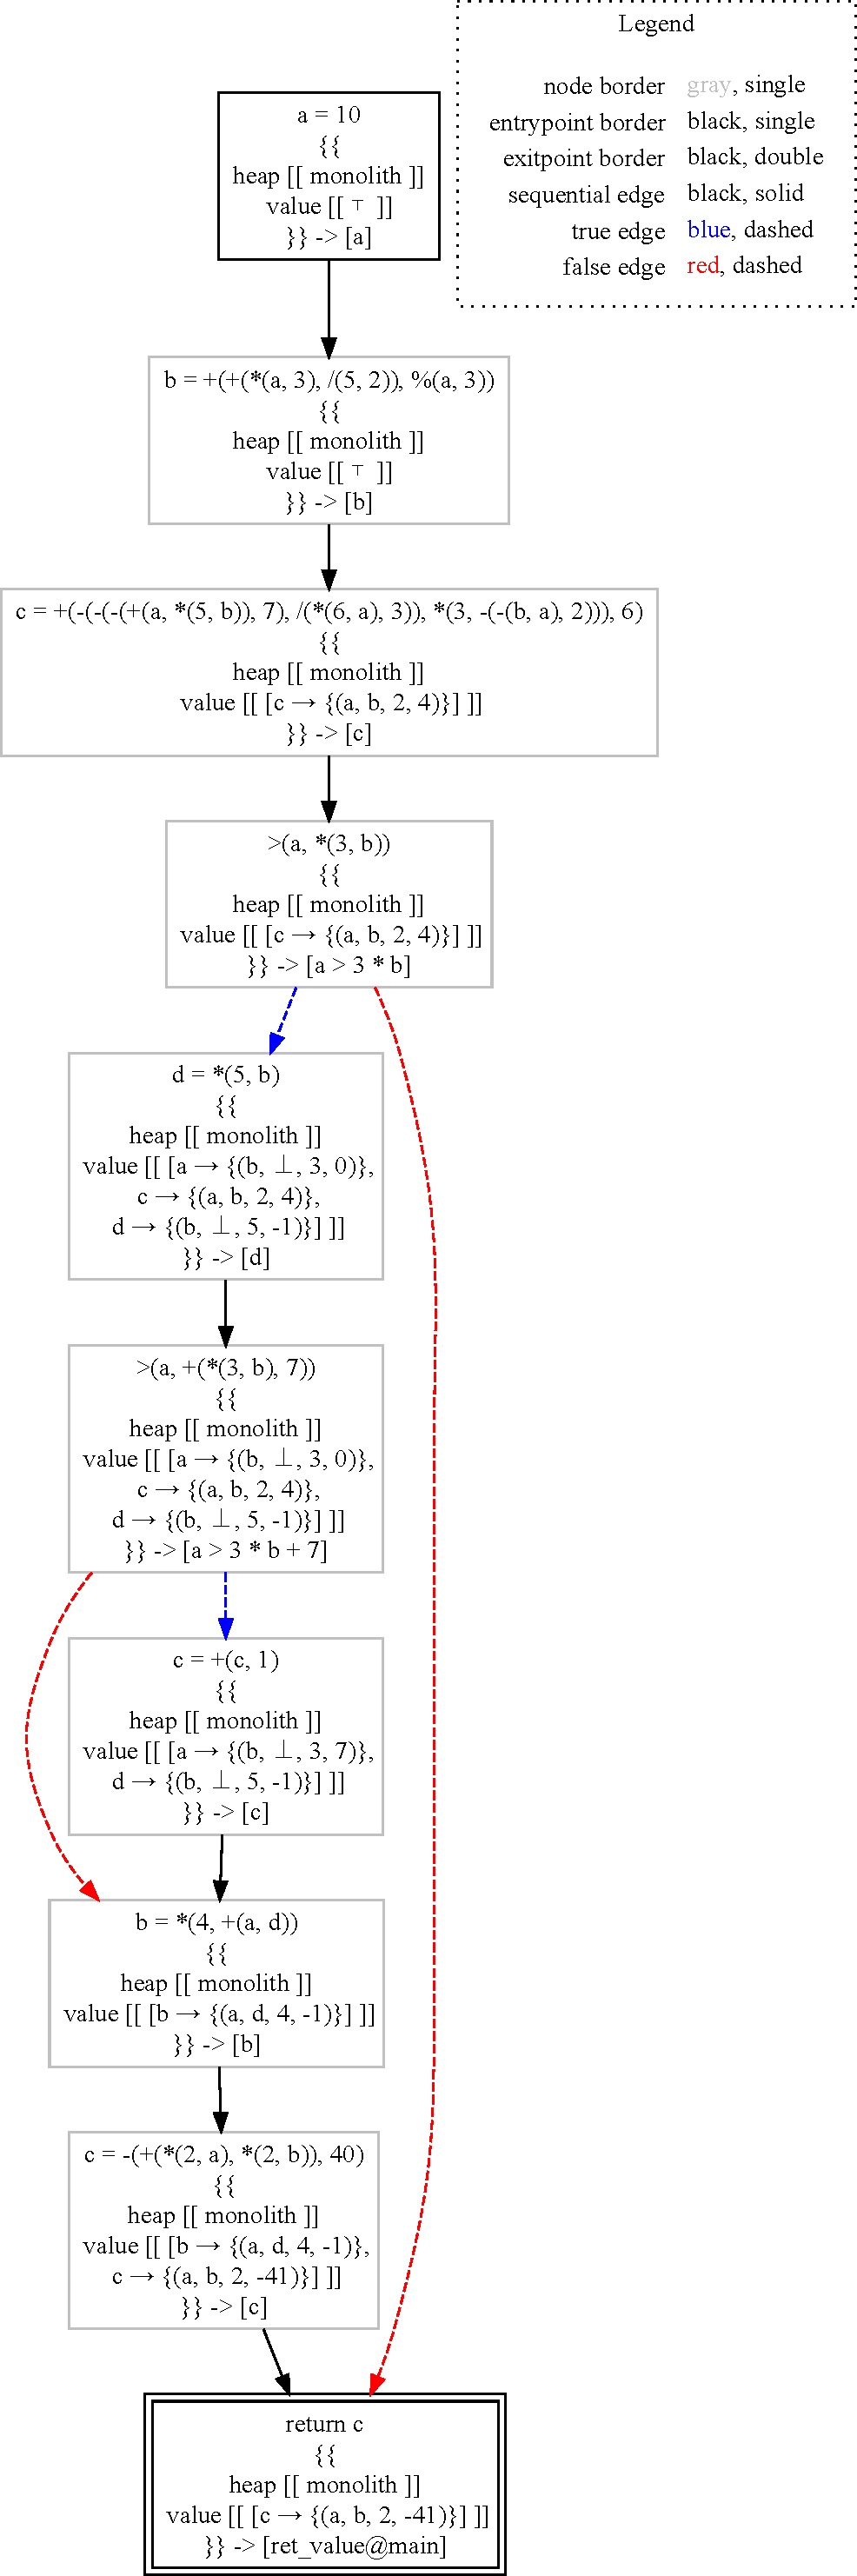
\includegraphics[width=0.15\textwidth]{test1.pdf}
    \caption{Output of the first test}
\end{figure}

%\noindent
Line \linenum{3} contains an assignment that assigns a constant value which cannot be turned in normalized form (see equation \ref{constr_formula}). Therefore, it is not tracked.

%\noindent
Line \linenum{4} contains an assignment that assigns an expression that cannot be simplified due to the factor \texttt{a\%3}, so it is not tracked.

%\noindent
Line \linenum{5}, once simplified, becomes the assignment \texttt{c = 2*(a+b)+5}, so, we can extract the constraint $\constraint{a}{b}{2}{4}$ associated to the variable \texttt{c}.

%\noindent
Line \linenum{7} contains a condition that is proved to be neither always true nor always false because variables \texttt{a} and \texttt{b} are not tracked.
Therefore, we can refine the abstract state inside the \texttt{if} block by adding the constraint $\constraint{b}{\perp}{3}{0}$ associated to variable $a$.

%\noindent
Line \linenum{8} contains an assignment that can be tracked, adding the constraint $\constraint{b}{\perp}{5}{-1}$ associated to variable \texttt{d}.

%\noindent
Line \linenum{9} contains another condition. Again, we cannot tell if the condition is either always true or always false, thus we refine the abstract state inside the \texttt{if} block. In this case, the new constraint $\constraint{b}{\perp}{3}{7}$ is more specific than $\constraint{b}{\perp}{3}{0}$ extracted on line \linenum{7}, so the latter is substituted by the former, and this can be seen on line \linenum{10}.

%\noindent
Line \linenum{10} contains an assignment but, since the assigned expression mentions the variable the expression is assigned to, that assignment is not tracked.
When exiting the \texttt{if} block of line \linenum{11}, the condition on line \linenum{9} is not true anymore, so the added constraint is deleted restoring the constraint extracted on line \linenum{7}.

%\noindent
Line \linenum{12} and \linenum{13} contain assignments that can be tracked as $\constraint{a}{d}{4}{-41}$ and $\constraint{a}{b}{2}{-1}$ respectively.

%\noindent
Line \linenum{14} closes the \texttt{if} block. Several operations are performed:
\begin{itemize}
    \item Variable \texttt{d} goes out of scope. Therefore every constraint associated to that variable and every constraint that mention that variable are deleted;
    \item The condition on line \linenum{7} is not true anymore. Therefore all the constraints extracted from that condition are deleted;
    \item The constraints tracked at the end of the \texttt{if} block are joined with the ones tracked before such block. This operation keeps the intersection of the constraints (i.e., the constraints that have the same values for $x$, $y$, $z$ and $k_1$ on both states. The value for $k_2$ is the lowest $k_2$ value among the aforementioned constraints).
\end{itemize}

\noindent
Line \linenum{15} contains a return statement, whose state reflects what was just said.

\subsection{New constraints on assignment}
% Molti assegnamenti + while con condizione non sempre vera/falsa
\begin{lstlisting}
class Test {
    main() {
        def a = 5;
        def b = 3;
        def c = 2*(a + b) + 1;
        def d = (-c) + 1;
        def e = 2*(-c) + 7;
        def f = 4*(-c) + 14;
        def g = a - b - 4;
        def v1 = a;
        a = b+c;
    }
}
\end{lstlisting}

Lines \linenum{3} and \linenum{4} contain assignments that are not tracked, since they assign constant values.

Line \linenum{5} can be tracked as usual. The new constraint $\constraint{a}{b}{2}{0}$ is added to the abstract state.

Line \linenum{6} can be turned into the normalized form (see equation \ref{constr_formula}). Therefore it creates the constraint $\constraint{c}{\perp}{-1}{0}$. Moreover, we can flip the assignment (as seen in \ref{reverse_assignement}) so that it becomes \texttt{c = -d + 1}, generating the new constraint $\constraint{d}{\perp}{-1}{0}$ associated to \texttt{c}.

Line \linenum{7} mentions again variable \texttt{c}. Since the assigned expression is a multiple (excluding the constant value) of the one assigned to \texttt{d}, we can rewrite the assignment as \texttt{e = 2d+5}, creating the constraint $\constraint{d}{\perp}{2}{4}$ (as seen in \ref{common_expressions}), that is added to the usual $\constraint{c}{\perp}{-2}{6}$, both associated to variable \texttt{e}.

Line \linenum{8} is an assignment that assigns an expression to variable \texttt{f}. By substituting variable \texttt{e} with the expression assigned to it, we end up with the assignment \texttt{f = 4*d + 10}, which generates the constraint $\constraint{d}{\perp}{4}{9}$ associated to variable \texttt{f}. Of course, as all the other assignments, we extract the constraint $\constraint{c}{\perp}{-4}{13}$ associated to \texttt{f}.

Line \linenum{9} is an example of the exception assignment (see \ref{exception}). The extracted constraint will be $\constraint{g}{b}{1}{3}$ associated to variable \texttt{a}.

Line \linenum{10} is a simple assignment.

Line \linenum{11}, instead, is an example of assignment propagation (see \ref{assignment_prop}). Therefore, we generate the new  constraint $\constraint{b}{c}{1}{-1}$ associated to variable \texttt{v1}.


%main() {
%    def a = 5;
%    def b = 3;
%    def c = 2*(a + b) + 1 --> Caso normale
%    def d = -c + 1; --> primo caso
%    def e = 2*d + 1; --> secondo caso
%    def f = 4*d - 2; --> secondo caso bis
%    def g = a - b; --> eccezione
%}

\begin{figure}[H]
    \centering
    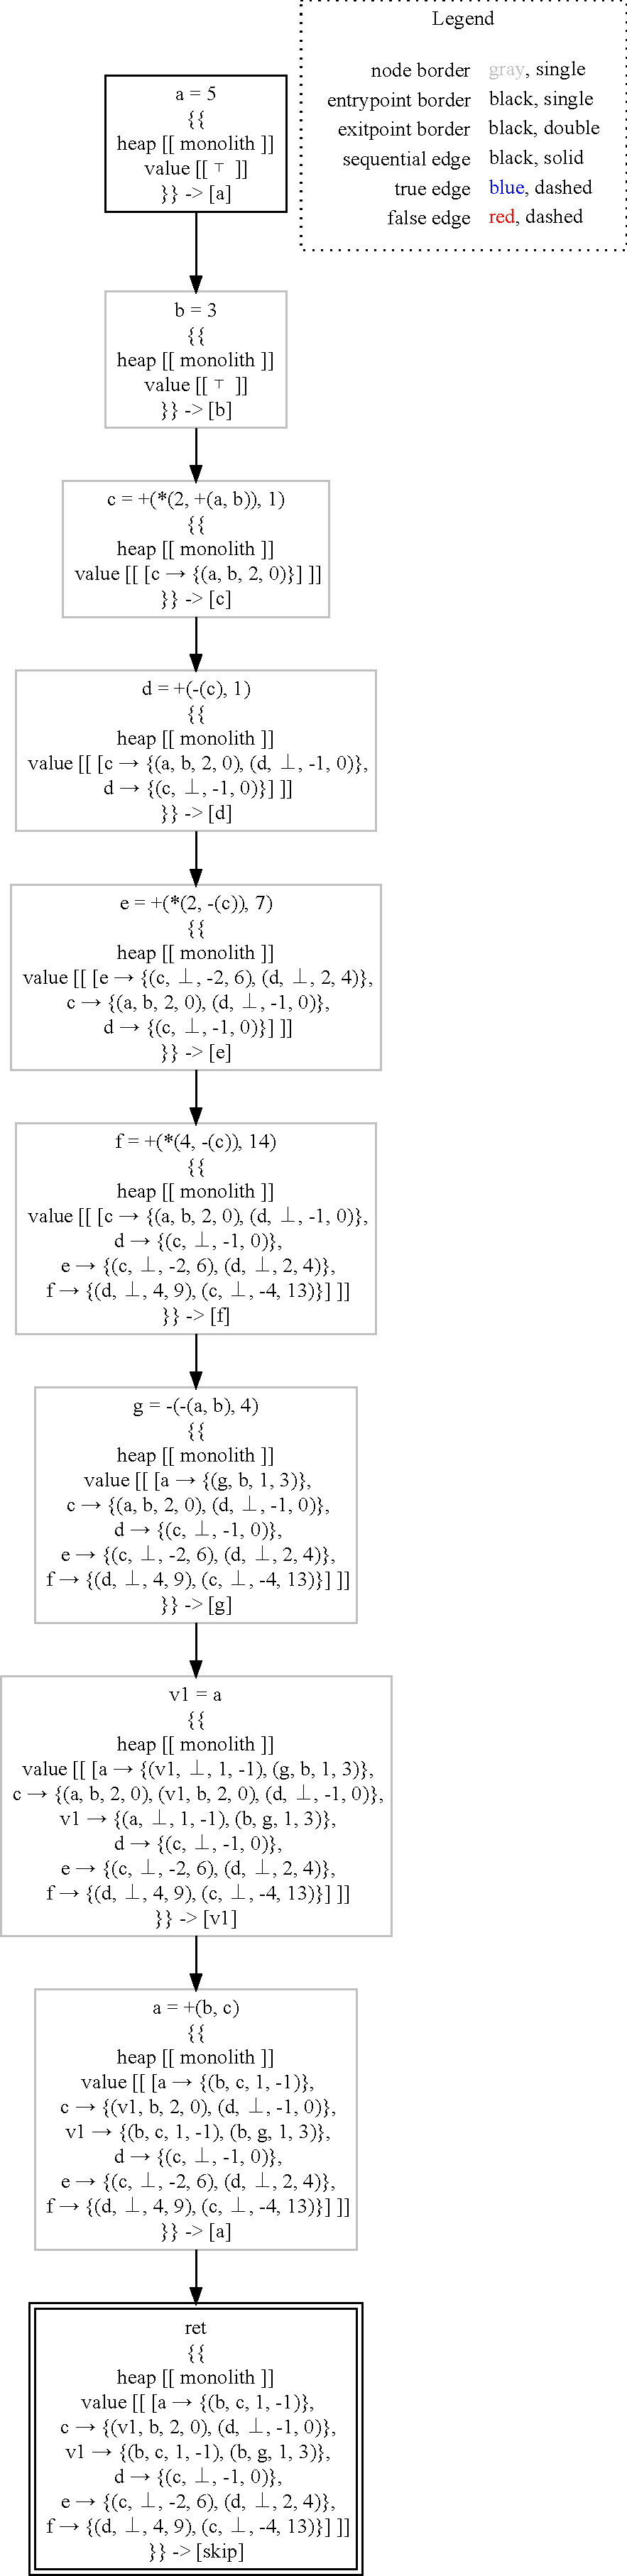
\includegraphics[width=0.14\textwidth]{test2.pdf} %0.23
    \caption{Output of the second test}
\end{figure}

\subsection{Conditions always true/false}
% Misto di if+while+for con condizioni sempre vere/false/boh
\begin{lstlisting}
class Test {
    main() {
        def a = 10;
        def b = 2*a + 7;
        if (b > a+a+4) {
            a = 2*b;
        } else {
            a = 7050*b;
        }
        def d = a+b;
        while ((d < a+b-9 && a < 5*3) ||                 (d <= a+b-5)) {
            d = d*2;
        }
        return d;
    }
}
\end{lstlisting}

Line \linenum{3} contains a non-trackable assignment while line \linenum{4} does.

\noindent
Line \linenum{5} contains a condition that can be proved to be always true. Indeed the \texttt{else} block will be skipped and the abstract state of all the instructions in the \texttt{else} block is $\perp$.

\noindent
Line \linenum{10} contains an assignment that can be tracked.

\noindent
Line \linenum{11} contains a condition that evaluates always to false. Therefore, no instruction of the while block is ever executed.
This fact is reflected on line \linenum{12} where the variable \texttt{d} is still tracked.


%main() {
%    def a = 10;
%    def b = 2*a + 7;
%    if (b > a+a+4) { --> Sempre vero
%        a = 2*b;
%    } else {
%        a = 7050*b;
%    }
%    def d = a+b;
%    while ((d < a+b-9 && a < 5*3) ||  
%            (d <= a+b-5)) { --> sempre false
%        d = d*2;
%    }
%    return d;
%}

\begin{figure}[H]
    \centering
    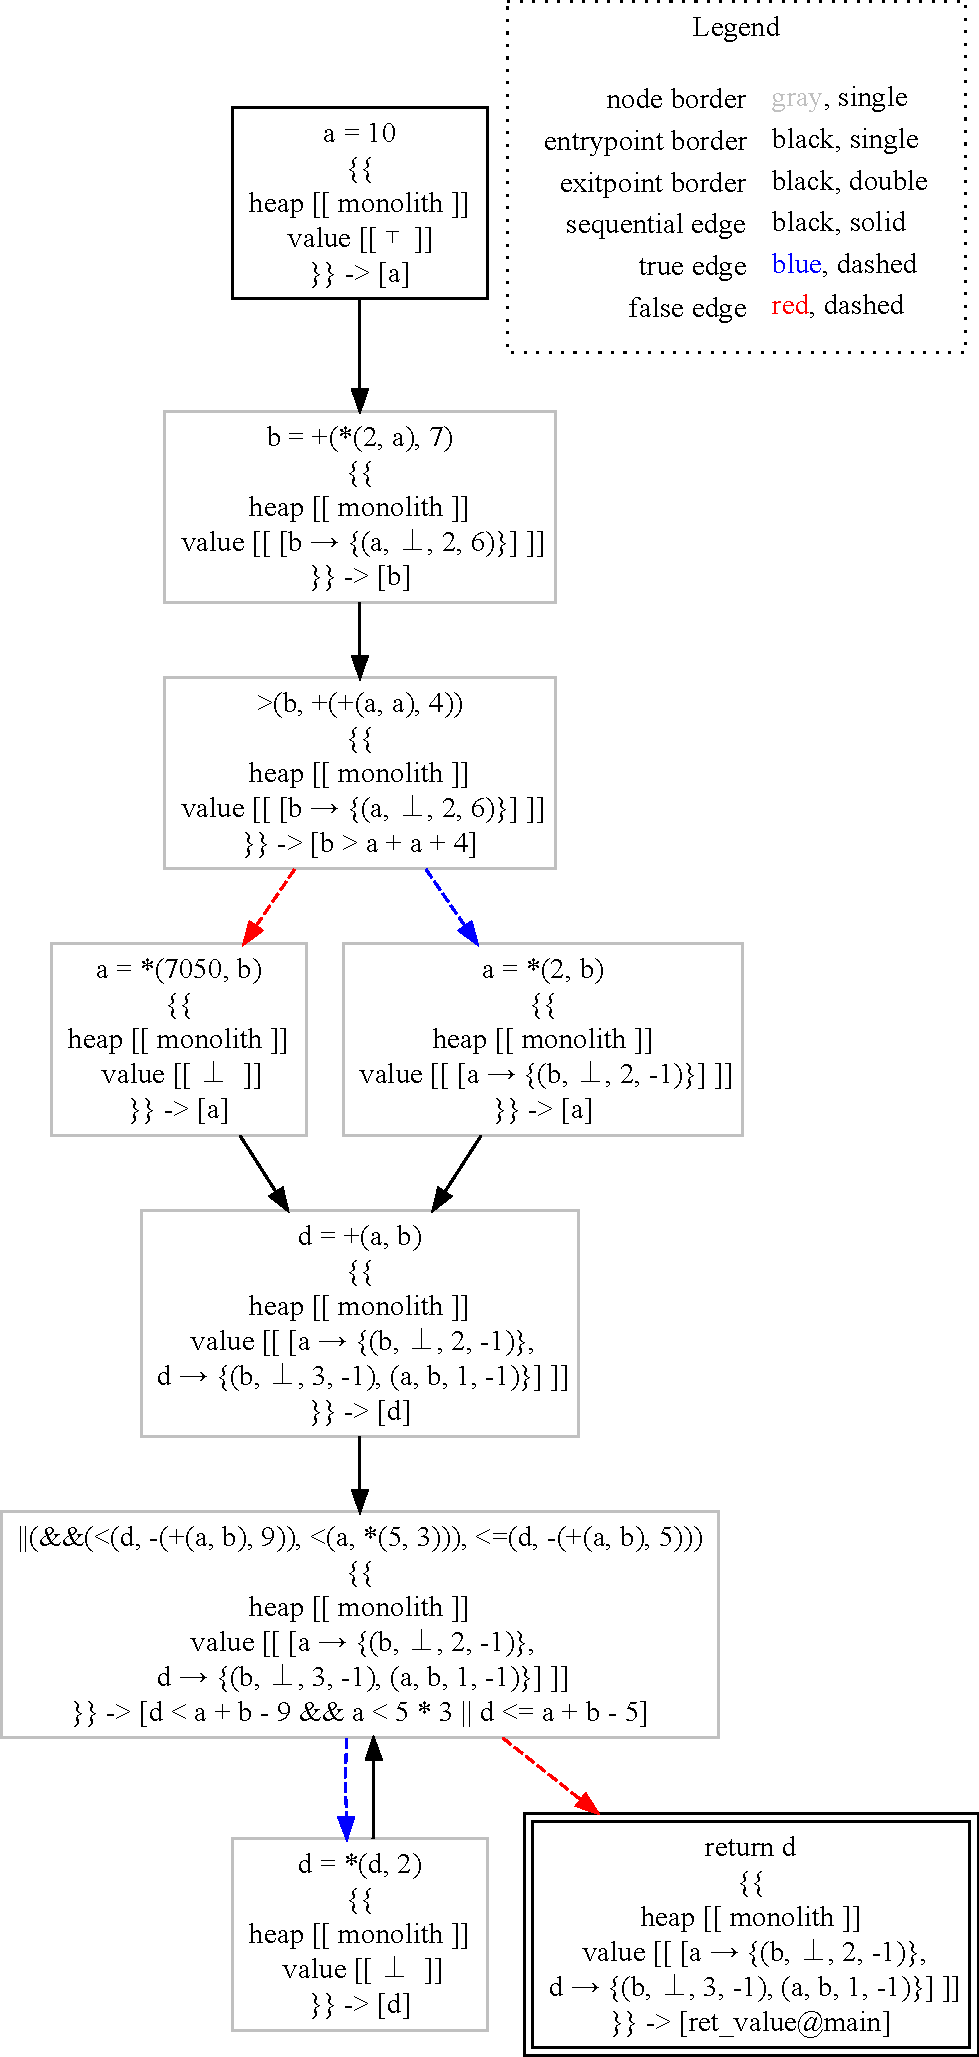
\includegraphics[width=0.25\textwidth]{test3.pdf}
    \caption{Output of the third test}
\end{figure}


%\section{Conclusion?}

\printbibliography

\end{document}